% Write the full path to the location of the graphics relative to book.tex
\graphicspath{{chapters/chp1/graphics/}}

\title{The FEniCS Project on AWS Graviton3}
\titlerunning{The FEniCS Project on AWS Graviton3}

\author{M.~Habera and J.~S.~Hale}
\authorrunning{Habera and Hale}

\institute{M.~Habera \email{michal.habera@rafinex.com} \at Rafinex SARL, Luxembourg and Institute of Computational Engineering, Department of Engineering, Faculty of Science, Technology and Medicine, University of Luxembourg, Luxembourg.\\
J.~S.~Hale \email{jack.hale@uni.lu} \at Institute of Computational Engineering, Department of Engineering, Faculty of Science, Technology and Medicine, University of Luxembourg, Luxembourg.}

\maketitle

\abstract{
We show performance results executing the FEniCS Project finite element
software on Amazon Web Services (AWS) c7g and c7gn instances with Graviton3
processors. Graviton3 processors implement the on the ARMv8.4-A instruction set and
provide Scalable Vector Extensions (SVE) for single instruction, multiple data
(SIMD) operations. Comparing clang 18 and GCC 13 series compilers for compiling
a high-order Laplace finite element kernel our results show that GCC emitted
more automatically vectorised loops than clang. The runtime performance of the
GCC compiled kernel was 20 \% faster than the clang compiled kernel. The c7gn
instances include a Elastic Fabric Adaptor (EFA) interconnect with a bandwidth
of $\SI{200}{\giga\byte\per\second}$ for low-latency and high-bandwidth Message
Passing Interface (MPI) based parallel communication.  We tested multi-node
weak scalability of a Poisson solver up to 512 MPI processes. We find the
overall performance and weak scalability of the c7gn-based cluster is similar
to a dedicated AMD EPYC Rome x86-64 cluster installed at the University of
Luxembourg.
}

\section*{Introduction}

The FEniCS Project~\cite{alnaes2015fenics,baratta_dolfinx_2023} has been used
to write finite element solvers for problems arising in fields that involve the
solution of partial differential equations (PDEs), including mathematics, biology,
physics, engineering, geophysics and mechanics.

AWS Graviton3-based instances aim to provide a cost effective compute resources
with a focus on scientific computing and machine-learning applications.
Particularly appealing for running scientific computing codes such as the
FEniCS Project is Graviton3's support for Scalable Vector Extension (SVE)
instructions and instances including an Elastic Fabric Adaptor (EFA)
interconnect for high-bandwidth low-latency communications between instances.

A key technology in the FEniCS Project is the use of automatic code generation
(compilation) to reduce the tedious and error-prone work associated with
building a finite element solver for a particular PDE. The user expresses their
finite element problem in the Unified Form Language
(UFL)~\cite{alnaes_unified_2014} and then the FEniCSx Form Compiler
(FFCx)~\cite{kirby_compiler_2006} translates the UFL description of the problem
into a low-level C kernel that computes the finite element tensor on any given
cell of the finite element mesh of the problem domain.

One  aspect of strong kernel performance at runtime is ensuring the assembly
code of the compiled kernel contains calls to single instruction multiple data
(SIMD) operations. SIMD operations can apply the same operation to multiple
data items. Widely available SIMD standards include Streaming SIMD Extensions
(SSE), Advanced Vector Extensions (AVX), Neon and Scalable Vector Extensions
(SVE). 

Ensuring that the compiled kernels contain SIMD instructions can be acheived in
a number of different ways. One option is to include compiler intrinsics in the
generated C code that directly call platform-specific SIMD operations. This can
provide excellent performance, but is inherently non-portable across SIMD
standards. Another option is to use a portable SIMD abstraction library e.g.
Google's Highway or SIMD Everywhere, that provides portable SIMD-like
abstractions on top of compiler intrinsics. A third option, and the one
currently used by FEniCSx, is to ensure that the generated C code is amenable
to the compiler applying automatic vectorisation, a process that automatically
converts a scalar program into a vectorised program.
 
Consequently to achieve good performance on Graviton3 it is important to verify
that the latest compilers do automatically emit ARM SIMD instructions (Scalable
Vector Extensions (SVE) and/or Neon) when compiling the generated C finite
element kernels and additionally that these kernels acheive reasonable runtime
performance. 

In addition to SIMD parallelisation at the kernel level, DOLFINx, the finite
element problem solving environment of the FEniCS Project, also supports
shared-memory parallel assembly of global finite element data structures
(sparse matrices and vectors) using the Message Passing Interface (MPI). The
finite element mesh is partitioned between MPI processes and each process is
responsible for assembling contributions from its own partition of the mesh.
Communication between MPI processes is then required to ensure a consistent
representation of the finite element linear system at degrees of freedom
located at the partition boundaries.



\section*{Methodology and Results}
In this section we present benchmark results. AWS c7g instances are compared to
Aion computing instances available at the University of Luxembourg HPC
facilities \cite{VCPKVO_HPCCT22}. These instances have different hardware
configuration, see \autoref{tab:aion-aws-config}. The purpose of the comparison
to ascertain an ARM-based cloud compute cluster can be broadly competitive with
a relatively modern x86-64 cluster.

The FEniCS Project components are written in a mixture of Python, modern-style
C++20 and Standard C17. All computationally intensive parts (core data
structures and algorithms for finite element linear system assembly) of DOLFINx
are written in a mixture of C++20 and Standard C17.


\begin{table}
  \footnotesize
  \renewcommand{\arraystretch}{1.5}
  \begin{tabular}{l|l|l}
                              & Aion node                                                          & AWS c7g instance \\ \hline \hline
    Processor                 & \makecell[l]{2 x (AMD Epyc ROME 7H12, \\ 64 cores @ 2.6 GHz)}      & \makecell[l]{1 x (Graviton3, \\ 64 cores @ 2.6 GHz)} \\ \hline
    Architecture              & x86\_64, Zen 2 (AVX2)                                              & ARMv8.5, Neoverse V1 (SVE) \\ \hline
    Memory                    & \makecell[l]{256 GB DDR4 \\ 3200 MT/s = 25.6 GB/s \\ 8 NUMA nodes} & \makecell[l]{128 GB DDR5 \\ 4800 MT/s = 38.4 GB/s \\ Unified Memory Access (no NUMA) } \\ \hline
    Total mem. bandwidth      & 2 x 200 GB/s                                                       & 1 x 300 GB/s \\ \hline
  \end{tabular}
  \vspace{5pt}
  \caption{Configuration of the Aion nodes (University of Luxembourg HPC) and AWS c7g (Amazon) instances. The c7gn instance used in the weak scaling tests additionally includes a $\SI{200}{\giga\byte\per\second}$ interconnect.}
  \label{tab:aion-aws-config}
\end{table}

\subsection*{Memory bandwidth}

Low-order finite element methods are typically memory bandwidth constrained as
the time taken to load and store data from main memory (e.g. the mesh geometry)
dominates the time taken to perform the arithmatic operations to compute the
finite element cell tensor itself. Understanding the memory bandwidth
characteristics of a processor is therefore important for ensuring optimal
performance.

STREAM and STREAM MPI \cite{McCalpin1995,McCalpin2007} are the industry standard
benchmarks for measuring sustained memory bandwidth performance. It estimates
memory bandwidth from memory intense operations (copy, scale, add) on large
arrays. In \autoref{fig:stream-single} results for the copy operation for
single-node benchmark are shown. For the single-node benchmark theoretical peak
memory bandwidth of $\SI{400}{\giga\byte\per\second}$ for Aion and
$\SI{300}{\giga\byte\per\second}$ for AWS c7g are reached within 80 \%, which is
considered a reasonable outcome of the STREAM benchmark. Bandwidth saturation is
observed around 20 \% of the node utilisation. Both curves show different
characteristics of the saturation point due to different memory access
configuration. On the Aion instances there are 8 non-unified memory access
(NUMA) nodes of 16 cores each, while AWS c7g was setup with unified memory
access.

In terms of multi-node scalability, low utilisation (8 processes on 8 nodes
each) helps to escape the bandwidth limitations as expected, see
\autoref{fig:stream-multiple}.

\begin{figure}
    \begin{subfigure}{.5\textwidth}
        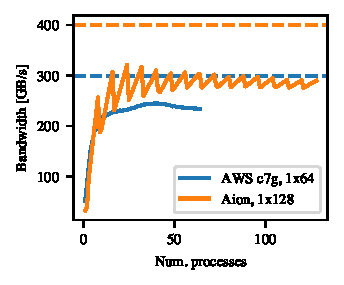
\includegraphics{chapters/chp1/graphics/stream_plots/stream_single_node.pdf}
        \caption{Single-node.}
        \label{fig:stream-single}
    \end{subfigure}%
    \begin{subfigure}{.5\textwidth}
        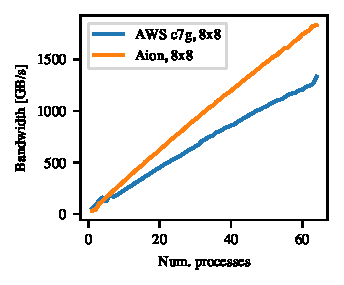
\includegraphics{chapters/chp1/graphics/stream_plots/stream_multi_node.pdf}
        \caption{Multi-node.}
        \label{fig:stream-multiple}
    \end{subfigure}
    \caption{STREAM benchmark.}
\end{figure}

\subsection*{Finite element kernels}

In order to measure the performance of a standard FEniCS user finite element
code we used the Local Finite Element Operator Benchmarks repository
\cite{Baratta2023}. The benchmark measures execution time for local finite
element kernel generated by the FEniCS Form Compiler (FFCx), \cite{Habera2020}.
Two types of kernels were generated for the purpose of this paper. Matrix-free
three-dimensional laplace kernel represents a finite element discretisation of
the action of laplace (stiffness) operator with spatially varying material
property $\kappa(x)$, i.e.
\begin{align}
    v_i = A_{ij} w_j, \quad
    A_{ij} = \int_K \kappa J_{mk} J_{mn} \nabla_k \phi_i \nabla_n \phi_j |\det J| \mathrm dx,
\end{align}
where $K$ is a fixed reference tetrahedron, $w_j \in \mathbb{R}^{n}$ is a fixed,
prescribed vector and $J$ is a Jacobian transformation matrix. The generated
kernel assembles a double precision vector $v_i \in \mathbb{R}^{n}$, where $n =
4$ for first-order discretization (low-order) and $n = 165$ for eight-order
discretization (high-order). Low-order kernels are expected to be memory
bandwidth limited, while high-order kernels have higher arithmetic intesity. In
addition, the matrix-free version requires fewer copy operations in comparison
to the assembly of a matrix, increasing the ratio of floating-point operations
to memory loads and stores. Consequently for the high-order kernels there is
the scope for significant performance increases if the compiler can
automatically emit SIMD instructions.

\subsubsection*{Generated code structure}

Compiler (loop) SIMD auto-vectorization is usually performed for inner-most loops
with compile-time known bounds. The analysis of FFCx autogenerated code is
required to understand the potential and missed optimizations.

\lstset{style=CStyle}
\begin{lstlisting}[language=c,
    caption=FFCx generated finite element kernel.,
    basicstyle=\ttfamily\footnotesize,
    keywordstyle=\ttb\color{deepblue}\footnotesize,
    label=lst:c-code]
void kernel(double* restrict A, const double* restrict w, ...){
    // 1. Static arrays of basis functions and quadrature weights.
    // 2. Quadrature rule independent computations.
    // 3. Quadrature loop body.
    for (int iq = 0; iq < NUM_QUAD_POINTS; ++iq) {
        // 3.1 Coefficient evaluation.
        for (int ic = 0; ic < NUM_DOFS; ++ic){
            w1_d100 += w[4 + (ic)] * FE0_C0_D100_Q530[0][0][iq][ic];
            // ...
        }

        // 3.2 Scalar graph evaluation.
        double sv_530_0 = w1_d100 * sp_530_18;
        double sv_530_1 = w1_d010 * sp_530_22;
        // ...

        // 3.3 Tensor assignment loop.
        for (int i = 0; i < NUM_DOFS; ++i) {
            A[(i)] += fw0 * FE0_C0_D100_Q530[0][0][iq][i];
            // ...
    }}
}
\end{lstlisting}

An example generated C code is shown in Code Listing \ref{lst:c-code}. Firstly,
there are arrays defining finite element basis functions at quadrature points
and have no arithmetic operations. Computations independent on the quadrature
loop contain more intense arithmetic operations (e.g. determinant of the
jacobian), but are executed only once.

The most critical part of the code is contained in the quadrature loop body. For
the eight-order laplace operator there is \lstinline{NUM_QUAD_POINTS = 214} and
\lstinline{NUM_DOFS = 165}. There are two inner-most loops with vectorization
potential: coefficient evaluation and tensor assignment. Both contain a set of
multiply-add operations.

Different compilers and compiler options were used to assess the performance
differences on the AWS c7g instances, see \autoref{tab:compilers-kernels}.

\begin{table}
    \centering
    \footnotesize
    \renewcommand{\arraystretch}{1.5}
    \begin{tabular}{l|l|l|l}
                                    & Compiler     & Aion                                                                                            & AWS c7g \\ \hline \hline
        Ofast, native, vectorized   & gcc 13.2.0   & \makecell[l]{-Ofast \\ -march=znver2 \\ -mtune=znver2}                                          & \makecell[l]{-Ofast \\ -mcpu=neoverse-v1} \\ \hline
                                    & clang 18.1.3 & \makecell[l]{-Ofast \\ -march=znver2 \\ -mtune=znver2}                                          & \makecell[l]{-Ofast \\ -mcpu=neoverse-v1} \\ \hline
        Ofast, native, no vec.      & gcc 13.2.0   & \makecell[l]{-Ofast \\ -march=znver2 \\ -mtune=znver2 \\ -fno-tree-vectorize}                   & \makecell[l]{-Ofast \\ -mcpu=neoverse-v1 \\ -fno-tree-vectorize} \\ \hline
                                    & clang 18.1.3 & \makecell[l]{-Ofast \\ -march=znver2 \\ -mtune=znver2 \\ -fno-slp-vectorize \\ -fno-vectorize}  & \makecell[l]{-Ofast \\ -mcpu=neoverse-v1 \\ -fno-slp-vectorize \\ -fno-vectorize} \\ \hline
        O2, no vec.                 & gcc 13.2.0   & \makecell[l]{-O2 \\ -fno-tree-vectorize}                                                        & \makecell[l]{-O2 \\ -fno-tree-vectorize} \\ \hline
                                    & clang 18.1.3 & \makecell[l]{-O2 \\ -fno-slp-vectorize \\ -fno-vectorize}                                       & \makecell[l]{-O2 \\ -fno-slp-vectorize \\ -fno-vectorize} \\ \hline
    \end{tabular}
    \vspace{5pt}
    \caption{Compiler versions and compilation flags used for finite element kernel benchmarks.}
    \label{tab:compilers-kernels}
\end{table}

For the finite element kernel benchmarks we compiled the kernels with
LLVM/clang 18.1.3 and GCC 13.2.0 for the purpose of comparing the generated
assembly code and comparing runtime performance.

Results for kernel benchmarks are included in \autoref{fig:local-deg1} and
\autoref{fig:local-deg8}. Low-order kernels show no dependence on compiler
vectorization setup. On the other hand, AWS c7g shows 1.3x speed-up over
Aion due to higher memory bandwidth for a single process (DDR5 vs. DDR4).

High-order kernels, which are expected to benefit from compiler optimization,
show this trend clearly. Both Clang and GCC auto-vectorizers perform well,
producing a noticeable speed-up (\textgreater 2x) in the most optimized setting. The
vectorization speed-up (\textgreater 4x) is more significant of the Aion instance.

\begin{figure}
    \begin{subfigure}{.5\textwidth}
        \centering
        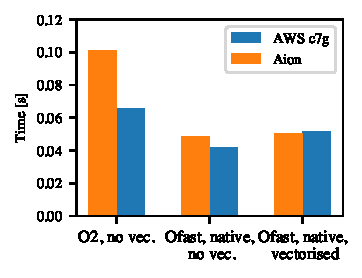
\includegraphics{chapters/chp1/graphics/kernel_plots/local_operator_clang_deg1.pdf}
        \caption{Clang 18.1.3.}
        \label{fig:local-clang-deg1}
    \end{subfigure}%
    \begin{subfigure}{.5\textwidth}
        \centering
        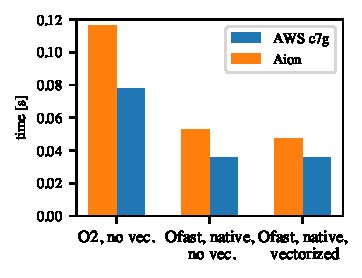
\includegraphics{chapters/chp1/graphics/kernel_plots/local_operator_gcc_deg1.pdf}
        \caption{GCC 13.2.0.}
        \label{fig:local-gcc-deg1}
    \end{subfigure}
    \caption{Low-order Laplace operator assembly.}
    \label{fig:local-deg1}
\end{figure}

\begin{figure}
    \begin{subfigure}{.5\textwidth}
        \centering
        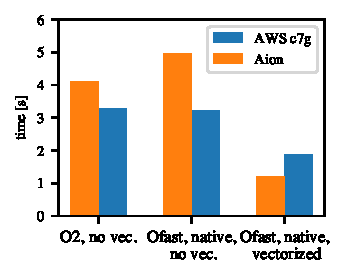
\includegraphics{chapters/chp1/graphics/kernel_plots/local_operator_clang_deg8.pdf}
        \caption{Clang 18.1.3.}
        \label{fig:local-clang-deg8}
    \end{subfigure}%
    \begin{subfigure}{.5\textwidth}
        \centering
        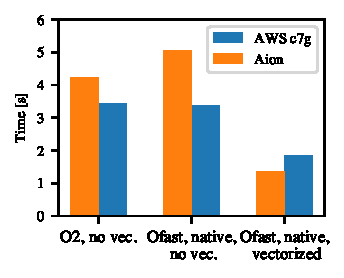
\includegraphics{chapters/chp1/graphics/kernel_plots/local_operator_gcc_deg8.pdf}
        \caption{GCC 13.2.0.}
        \label{fig:local-gcc-deg8}
    \end{subfigure}
    \caption{High-order Laplace operator assembly.}
    \label{fig:local-deg8}
\end{figure}

Optimization reports (\texttt{-Rpass=loop-vectorize} for Clang,
\texttt{-fopt-info-vec-optimized}) for GCC and the inspection of the generated
assembly reveal:
\begin{itemize}
    \item On Graviton3, both GCC and Clang generate SVE FMLA and FMAD (fused
    Multiply-Add) instructions for both the coefficient evaluation and tensor
    assignment loops. Assembly excerpt for the coeffient evaluation is show
    below. As expected, there are two contiguous loads LD1D into two of the
    available SVE Z0-Z31 registers followed by a Multiply-Add instruction.
\begin{lstlisting}[
    basicstyle=\ttfamily\footnotesize,
    keywordstyle=\ttb\color{deepblue}\footnotesize]
ld1d    {z0.d}, p0/z, [x7, x0, lsl #3]
ld1d    {z25.d}, p0/z, [x3, x0, lsl #3]
fmla    z3.d, p0/m, z25.d, z0.d
...
faddv   d1, p1, z1.d
\end{lstlisting}
    The result is accumulated into an SVE register Z3 which is then horizontally
    summed outside of the vectorized loop. Here P0 is a predicate
    register without any constraints on the available elements.
    \item On Aion, both GCC and clang vectorize both coefficient evaluation and
    tensor assignment loops and rely on the \lstinline{VFMADD231PD} instructions
    on the YMM registers, i.e. vectorization width of 4 doubles.
    \item  We have verified that Graviton3 c7g instances offer the expected
    \SI{256}{bit} maximum vector width using \lstinline{svcntb()} function from
    the ARM C SVE header library. This matches the AVX2 vector width on the
    Aion instaces.
\end{itemize}

\subsection*{Parallel scalability}

Results for the parallel scalability were produced using performance test codes
for FEniCSx \cite{Wells2023} built against DOLFINx 0.6.0 and PETSc 3.18
\cite{petsc} with the Spack package manager using GCC 12.2.0. We setup Spack to
use a version of OpenMPI provided by AWS which includes the appropriate
libfabric with native support for the EFA interconnect.

The Poisson equation solver benchmark consists of the following measured steps:
\begin{enumerate}
    \item Create mesh. Create a unit cube mesh and discretise using linear
    tetrahedral cells. Partition the mesh with Parmetis partitioner and
    distribute.
    \item Create function space. Create a scalar-valued, globally $C^0$
    continuous, piecewise linear function space on the mesh.
    \item Assemble matrix. Execute the local Poisson equation kernel over the
    mesh and assemble into a PETSc MATMPIAIJ (distributed compressed sparse row)
    matrix.
    \item Solve. Run Conjugate Gradient (CG) solver with a classical algebraic
    multigrid (BoomerAMG \cite{hypre}) preconditioner.
\end{enumerate}
%
Weak scaling results (constant workload of approx. \SI{5e+5} degrees-of-freedom
per process) are shown in \autoref{fig:weak-scaling}. Both Aion and AWS c7gn
show almost constant times for mesh and function space creation. Moreover,
matrix assembly has the most ideal weak parallel scalability due to the
cell-local nature of the assembly loop and negligible amount of MPI
communication during matrix finalisation. The solve step shows small
increase (30 \%) for both clusters.

\begin{figure}
    \begin{subfigure}{.7\textwidth}
        \centering
        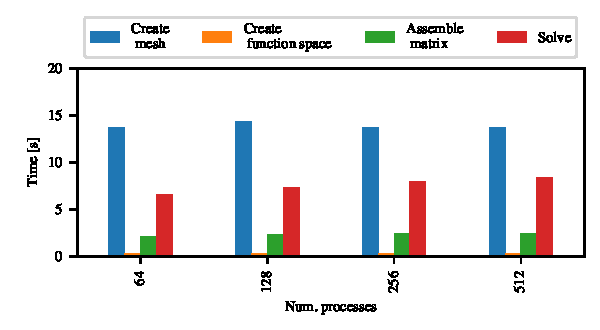
\includegraphics{chapters/chp1/graphics/parallel_scaling_plots/output/weak_scaling_aion_poisson.pdf}
        \caption{Aion, \SI{5e+5} degrees-of-freedom per process, 25 \% utilisation (32 processes per node).}
        \label{fig:weak-scaling-aion}
    \end{subfigure}

    \begin{subfigure}{.7\textwidth}
        \centering
        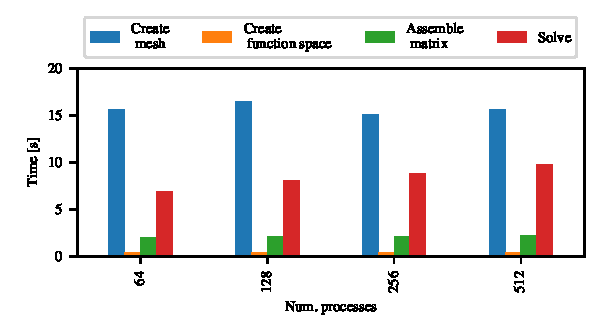
\includegraphics{chapters/chp1/graphics/parallel_scaling_plots/output/weak_scaling_aws_c7gn_poisson.pdf}
        \caption{AWS c7gn, \SI{5e+5} degrees-of-freedom per process, 50 \% utilisation (32 processes per node).}
        \label{fig:weak-scaling-aws}
    \end{subfigure}
    \caption{Weak parallel scalability of the Poisson equation solver.}
    \label{fig:weak-scaling}
\end{figure}

\section*{Conclusion}

Benchmarks for memory bandwidth, local finite element kernels and parallel
scalability of Poisson solver were executed on Aion nodes and on AWS c7g(n)
instances.

Memory bandwidth measured using STREAM MPI confirms higher memory transfer rate
of AWS c7g(n), but a superior total bandwidth of ~\SI{310}{\giga\byte\per\second}
per Aion node.

In terms of auto-vectorization capabilities of GCC and clang, both produced
optimized instructions for the targeted microarchitectures (Zen 2 for Aion and
Neoverse V1 for AWS c7g). This observation was confirmed with performance
benchmarks based on local finite element kernels for the Laplace
operator for low (memory bound) and high (compute bound) orders.

The MPI-based distributed memory Poisson equation solver shows good weak
scaling on the c7gn-based cluster, with results comparable to the in-house
University of Luxembourg Aion system.

Executing the FEniCS Project on ARM64, and more specifically on the Graviton3
CPU, has proved to be straightforward. There were no ARM64, or Graviton3,
specific adjustments required. Credit for this can largely be attributed to the
dedicated work of the Open Source community in ensuring that the entire HPC
toolchain is ready for the ARM64 transition, and the engineering work done by
AWS on their Graviton3-based instances.

\section*{Supplementary material}
Raw data and plotting scripts are archived at \cite{}.

\begin{acknowledgement}
This project has received compute resources from Amazon Web Services (AWS)
through the first and second collaborative University of Luxembourg and
AWS Graviton3 call.

This research was funded in whole, or in part, by the National Research Fund
(FNR), grant reference COAT/17205623. For the purpose of open access, and in
fulfillment of the obligations arising from the grant agreement, the author has
applied a Creative Commons Attribution 4.0 International (CC BY 4.0) license to
any Author Accepted Manuscript version arising from this submission.
\end{acknowledgement}

\bibliographystyle{spbasic}
\bibliography{chapters/chp1/bibliography.bib}


